\documentclass[fontsize=12pt]{article}
\usepackage[a4paper, margin=1in]{geometry}
\usepackage{hyperref}
\usepackage{graphicx}

\title{\textbf{Model for UHECR arrival directions}}

\begin{document}
\maketitle
 
I have implemented the model from \cite{soiaporn} in Stan, with some modifications due to the different approach to sampling. For convenience, I briefly summarise the model here, then show some recreated results which confirm the consistency of the two implementations. 

\section{Model}

The model is essentially a spatially-inhomogeneous poisson process where the rate is described by a mixture model over different putative source locations, including an isotropic background component. Following the formalism and notation of \cite{soiaporn} to facilitate comparison, the likelihood has the form:

\begin{equation}
\mathcal{L}(F_T, \mathbf{F}, \kappa) = e^{-\bar{N}} \prod_i \sum_k F_k f_{ik}
\end{equation}

Where $F_T$ is the total flux expected from all $k$ sources and the $k = 0$ background component, $f$ is the associated fraction, $\kappa$ is the deflection parameter of the source von-Mises Fisher distribution, $\bar{N}$ is the total number of expected events and the product is over all $i$ observed UHECR arrival directions.  The flux of each source is weighted its distance, assuming a ``standard candle'' luminosity distribution. Thus $F_k = fw_kF_T$ for $k \geq 1$ with $w_k = \frac{1/D_k^2}{\sum_j 1/D_j^2}$. The background flux is simply described by $F_0 = (1 - f) F_T$. UHECR are produced at the source locations, $\varpi_k$, then undergo magnetic deflections during propagation and have a finite detection uncertainty. Both deflections from the true position are modelled using the von-Mises Fisher distribution on the unit sphere, characterised by deflection parameters $\kappa$ and $\kappa_c$ for the magnetic defection and the detection uncertainty respectively. For ease of computation, it is possible to marginalise over the latent true arrival directions $\omega_i$, using the magnetic deflection distribution as a prior:

\begin{equation}
f_{ik} = \int d \omega_i p(d_i | \omega_i, \kappa_c) A_{\perp} (t_i, \omega_i) \rho(\omega_i | \varpi_k, \kappa) 
\end{equation}
where $d_i$ are the detected arrival directions and $A_{\perp}$ is the effective area in the direction of $\omega_i$. This integral can be solved analytically to give:

\begin{equation}
f_{ik} = A_i \cos(\theta_i) \frac{\kappa \kappa_c}{4 \pi \sinh(\kappa) \sinh(\kappa_c)} \frac{\sinh(|\kappa_c d_i + \kappa \varpi_k |)}{|\kappa_c d_i + \kappa \varpi_k |}
\end{equation}
where $A_i$ is the effective area of the observatory at time $t_i$, and $\theta_i$ it the incidence angle of the detected UHECR. 

To calculate $\bar{N}$ it is necessary to take into account the non-uniform exposure of the Pierre Auger observatory. The exposure can be simply modelled by considering a cone of reconstructable zenith angles within $60^{\circ}$ of the observatory zenith, which varies on the celestial sphere due to the Earth's rotation. The average exposure can be calculated by averaging over one sidereal day. This results in an exposure function $\epsilon(\omega)$ which is uniform in right acsension and is purely a function of declination. In order to calculate $\bar{N}$, we are interested in the convolution of this exposure function with the source distributions. This is given by:

\begin{equation}
\epsilon_k  = \int d \omega \rho(\omega | \varpi_k, \kappa) \epsilon(\omega)
\end{equation}

This integral cannot be solved analytically, but can be pre-computed for known source locations $\varpi_k$. In the Stan implementation, we want to infer $\kappa$ which cannot be factored out from this integral. As the variation of the integral with expected $\kappa$ values is well-behaved and relatively small, this can be achieved by 1D interpolation over a pre-computed grid over the integral value. 

The full details of the implementation can be found in the \href{https://github.com/cescalara/uhecr_model}{GitHub repository}.

\section{Comparison with the work of Soiaporn et al. (2012)}

The main differences between the full Stan implementation and that of \cite{soiaporn} are:

\begin{itemize}
\item $\kappa$ can be inferred simultaneously and is not conditioned on, as is the case with the Metropolis-within-Gibbs implementation
\item The priors for $f$ and $F_T$ are not constrained by the need to provide closed form conditional distributions for the Gibbs steps
\item The sampling in Stan is $\sim$ 10 times faster than a naive implementation of the Metropolis-within-Gibbs approach in python 
\item In the Stan implementation, the discrete latent parameters for the UHECR labels are marginalised over which allows for better exploration of the tails of the posterior distribution and more efficient sampling, as described in \cite{stan_manual}
\item The Stan model is easier to implement as it is not necessary to derive the conditional distributions or to have to design and verify a custom sampling algorithm   
\end{itemize} 

In order to make the comparison between the Stan model and the original, some changes are made to the full Stan implementation, which are described when necessary.

\subsection{Figure 4}

In order to recreate Figure 4 from \cite{soiaporn}, it was necessary to make $\kappa$ fixed to mimic the Metropolis-within-Gibbs implementation. An exponential prior was also used for $F_T$, as described in \cite{soiaporn}. The case of 17 AGN and all data-taking periods was considered (top-right in the original Figure 4). 

\begin{figure}[h]
\centering
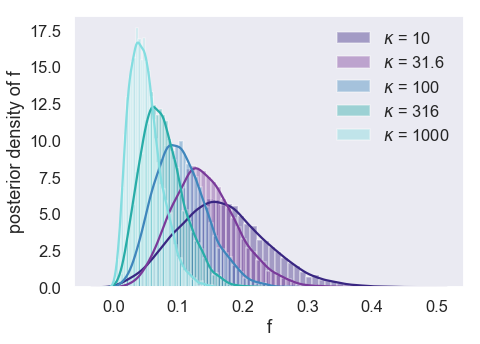
\includegraphics[width = 0.7\textwidth]{../notebooks/figures/soiaporn_fig4.png}
\caption{Posterior distributions for f, conditioned on $\kappa$ = 10, 31.6, 100, 316 and 1000.}
\end{figure}

\subsection{Figure 5}

In order to recreate Figure 5 from \cite{soiaporn}, $\kappa$ was left as a free parameter to mimic the approximate calculation of the marginal posterior of $\kappa$ using Chib's method, which is described in \cite{soiaporn}. An exponential prior for $F_T$ was used as well as a log-flat prior for $\kappa$. The case of 17 AGN and all data-taking periods was considered (top-right in the original Figure 5), as well as that for 17 AGN and only periods 2 and 3 (top-left in the original). 

\begin{figure}[h]
\centering
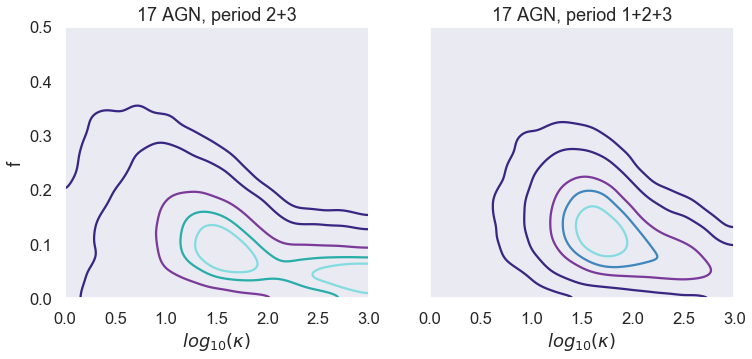
\includegraphics[width = \textwidth]{../notebooks/figures/soiaporn_fig5.png}
\caption{Joint marginal posterior distributions for $f$ and $\kappa$. The contours mark HPD credible regions of probability 0.25, 0.5, 0.75, 0.95 and 0.99, from light to dark colours respectively. The marginal posteriors were sampled with $\sim$ 15000 effective samples in each case.}
\end{figure}

\section{Conclusion}

The figures show good agreement between the two implementations. The notebook used to produced the figures can be found \href{https://github.com/cescalara/uhecr_model/blob/master/notebooks/auger2010_study.ipynb}{here}. In order to move forward and include the UHECR energies into the model, as well as to bring it closer to a physical description of UHECR phenomenology, the model as described here will be reparametrised in terms of source luminosities and a background flux. This will follow the ideas in \cite{watson, khanin}.

\begin{thebibliography}{9}

\bibitem{soiaporn} 
Soiaporn, K. et al., 2012. \emph{Multilevel Bayesian framework for modeling the production, propagation and detection of ultra-high energy cosmic rays}. arXiv.org, astro-ph.HE(3), pp. 1249-1285.

\bibitem{stan_manual}
The Stan development team, 2017. \emph{Stan Modeling Language User's Guide and Reference Manual}, Stan version 2.17.0. Ch 15.

\bibitem{watson}
Watson, L.J., Mortlock, D.J. \& Jaffe, A.H., 2011. \emph{A Bayesian analysis of the 27 highest energy cosmic rays detected by the Pierre Auger Observatory}. Mon. Not. Roy. Astron. Soc., 418(1), pp.206-213.

\bibitem{khanin}
Khanin, A. \& Mortlock, D.J., 2016. \emph{A Bayesian analysis of the 69 highest energy cosmic rays detected by the Pierre Auger Observatory}. arXiv.org, astro-ph.HE(3), pp.2765-2778.

\end{thebibliography}


\end{document}

